\documentclass[a4paper,11pt]{article}
\usepackage{graphicx,url}
\usepackage{draftwatermark}
\SetWatermarkText{DRAFT}
\SetWatermarkScale{8}
%\usepackage[big,compact,sf]{titlesec}
%\usepackage{sidecap}
\usepackage{graphics,graphicx}
%\usepackage{verbatim}
%\usepackage{wrapfig}
%\usepackage{floatflt}
%\usepackage{times}
%\usepackage{multicol}
\usepackage{color}
\newcommand{\red}{\textcolor{red}}

%\usepackage{sober}
%\usepackage[small,compact,sf]{titlesec}

\newcounter{fred}

\newcommand{\mic}{\mu{\rm m}}
\def\es{\mathrel{\rm e^-/s}}
\def\pix{\mathrel{\rm pix}}
\def\elec{\mathrel{\rm e^-}}
\def\kpc{\mathrel{\rm kpc}}
\def\Gpc{\mathrel{\rm Gpc}}
\def\Msol{\mathrel{\rm M_{\odot}}}
\def\fsub{\mathrel{f_{\rm sub}}}
\def\Mtot{\mathrel{M_{\rm tot}}}
\def\ls{\mathrel{\hbox{\rlap{\hbox{\lower4pt\hbox{$\sim$}}}\hbox{$<$}}}}
\def\gs{\mathrel{\hbox{\rlap{\hbox{\lower4pt\hbox{$\sim$}}}\hbox{$>$}}}}
\def\Msolpyr{\mathrel{\rm M_{\odot}\,yr^{-1}}}
\def\mas{\mathrel{\rm mas}}
\def\pc{\mathrel{\rm pc}}
\def\Ho{\mathrel{H_{\rm 0}}}
\def\oM{\mathrel{\Omega_{\rm M}}}
\def\oL{\mathrel{\Omega_{\rm \Lambda}}}
\def\kms{\mathrel{\rm km\,s^{-1}}}
\def\ms{\mathrel{\rm m\,s^{-1}}}
\def\m{\mathrel{\rm m}}
\def\nm{\mathrel{\rm nm}}
\def\mm{\mathrel{\rm mm}}
\def\cm{\mathrel{\rm cm}}
\def\km{\mathrel{\rm km}}
\def\um{\mathrel{\mu{\rm m}}}
\def\ang{\mathrel{\rm \AA}}
\def\Mpc{\mathrel{\rm Mpc}}
\def\ksec{\mathrel{{\rm ksec}}}
\def\mag{\mathrel{\rm mag}}
\def\Gyr{\mathrel{\rm Gyr}}
\def\Hz{\mathrel{\rm Hz}}
\def\MHz{\mathrel{\rm MHz}}
\def\GHz{\mathrel{\rm GHz}}
\def\THz{\mathrel{\rm THz}}
\def\PHz{\mathrel{\rm PHz}}
\def\EHz{\mathrel{\rm EHz}}
\def\Js{\mathrel{\rm Js}}
\def\J{\mathrel{\rm J}}
\def\W{\mathrel{\rm W}}
\def\eVs{\mathrel{\rm eV\,s}}
\def\eV{\mathrel{\rm eV}}
\def\K{\mathrel{\rm K}}
\def\Jy{\mathrel{\rm Jy}}
\def\mJy{\mathrel{\rm mJy}}
\def\uJy{\mathrel{\rm \mu Jy}}
\def\sr{\mathrel{\rm sr}}
\def\rad{\mathrel{\rm rad}}
\def\deg{\mathrel{\rm deg}}
\def\degsq{\mathrel{\rm deg}^2}
\def\fwhm{\mathrel{\rm FWHM}}
\def\fried{\mathrel{r_0}}
\def\fo{\mathrel{f_{\rm o}}}
\def\fe{\mathrel{f_{\rm e}}}
\def\s{\mathrel{\rm s}}
\def\dol{\mathrel{D_{\rm OL}}}
\def\dos{\mathrel{D_{\rm OS}}}
\def\dls{\mathrel{D_{\rm LS}}}


\newcommand{\captionfonts}{\small}
\makeatletter  % Allow the use of @ in command names
\long\def\@makecaption#1#2{%
  \vskip\abovecaptionskip
  \sbox\@tempboxa{{\captionfonts #1: #2}}%
  \ifdim \wd\@tempboxa >\hsize
    {\captionfonts #1: #2\par}
  \else
    \hbox to\hsize{\hfil\box\@tempboxa\hfil}%
  \fi
  \vskip\belowcaptionskip}
\makeatother   % Cancel the effect of \makeatletter


\setlength{\textwidth}{172mm} 
\setlength{\textheight}{260mm}
\setlength{\topmargin}{-20mm} 
\setlength{\oddsidemargin}{-5mm}
\setlength{\evensidemargin}{10mm} 
\setlength{\headheight}{5mm}
\setlength{\headsep}{5mm} 
\setlength{\hoffset}{0in}
\setlength{\voffset}{0in}

\parskip=2truemm                       % Paragraph spacing
\parindent=4truemm                       % Paragraph indentation

\begin{document}

\pagestyle{myheadings}\markright{LSST:UK Galaxy Clusters White Paper 2016}

\sloppy

\pagestyle{empty}

~\vspace{70mm}

\centerline{\LARGE\bf LSST:UK Galaxy Clusters}
\bigskip\bigskip\bigskip
\centerline{\Large\bf High Level Science Interests and Science Requirements}
\medskip
\centerline{\Large\bf of the UK Galaxy Clusters Community}
\medskip
\centerline{\Large\bf as they relate to LSST}
\bigskip\bigskip\bigskip
\centerline{\Large\bf White Paper 2016}

\vspace{90mm}

\large
\noindent{\bf Last updated}: June 16, 2016

\noindent{\bf Contributors}: Graham P.\ Smith, et al. {\it [add your names here]}


\newpage
\pagestyle{myheadings}
\setlength{\topmargin}{-10mm}
\setlength{\textheight}{255mm}

\tableofcontents

\newpage

\section{Introduction {\it [Responsible: Graham Smith]}}

The purpose of this document is to summarise and communicate the UK
galaxy cluster community's interests as they relate to future
exploitation of LSST.  Section 2 describes our interests and the high
level requirements that they place on LSST data and combining data
from LSST with data from other upcoming facilities, including
\emph{Euclid} and \emph{e-ROSITA}.  Section 3 distils the common
themes from our varied interests to form the basis for discussion with
other communities within LSST (both UK-based, and internationally),
and colleagues leading the development of other facilities.

It is also envisaged that this document, and the discussions that it
stimulates, will help to shape requests for funding for galaxy cluster
science in the future.  The LSST:UK Phase B proposal to STFC's PPRP
will be a key opportunity to secure funding to support the development
of computer algorithms that the UK community will need in order to
delivering world-class galaxy cluster science with LSST.

The initial names attached to science interests in Section 2 is based
on participation/discussion at the inaugural LSST:UK Clusters meeting
on June 7, 2016.  However this document is open for anyone in the UK
to join and contribute to.  The aim is to be succinct, so please try
to stick to no more than one page per science interest in Section 2.

We will need to add a section that discusses how our interests,
requirements on the data, and strengths compare with those of the US
community.

\section{Science Interests}

UK astronomers play leading international roles in numerous aspects of
galaxy cluster research that are relevant to the future exploitation
of LSST data.  

Recent highlights include constraints on the nature of dark matter
(Harvey et al.\ 2015, Sci, 347, 1462), measurements of intracluster
light at $z=1$ (Burke et al., 2012, MNRAS, 425, 2058), systematic
census of acticity in brightest cluster galaxies (Green et al.,
arXiv:1606.01251), cosmological hydrodynamical simulations that
reproduce the observed properties of galaxy clusters and groups
(McCarthy et al., 2016), testing chameleon gravity with clusters from
the XMM Cluster Survey (Wilcox et al., 2015, MNRAS, 452, 1171),
exploring the structure of cluster cores using Hubble Frontier Fields
observations (Jauzac et al., 2015, MNRAS, 452, 1437; Jauzac et
al.\ arXiv:1606.04527), galaxy evolution in clusters and groups (Sean
McGee, others), discovery of protoclusters around high-z radio
galaxies (Hatch et al., ...), X-ray scaling relations of clusters
(Giles et al.\ 2016, A\&A, 592, 3), weak-lensing calibration of the
masses of galaxy groups and clusters (Smith et al., 2016, MNRAS, 456,
L74; Okabe \& Smith, arXiv:1507.04493; Lieu et al.\ 2016, A\&A, 592,
4).

\emph{Explicitly mention surveys that we have leading roles in?  GEEC,
  GEEC2, XXL, CARLA, XCS, DES, GOGREEN, LoCuSS, ...}

The following sections outline the science interests of the UK's
galaxy cluster community as they relate to LSST, highlighting the
requirements that these interests place on LSST data.

\subsection{Intracluster Light and low surface brightness emission {\it [Responsible: Chris Collins]}}

Understanding the build up of stellar mass at the centres of galaxy
clusters is a key component to our understanding of galaxy
evolution. The centres of rich clusters are dominated by Brightest
Cluster Galaxies (BCG) which are the most luminous galaxies in the
universe emitting photospheric light. Observational studies have
consistently indicated that the masses of BCGs change by a factor no
larger than $30\%$ over the cosmic time out to a redshift $ z~1$, with
some results suggesting considerably less change (e.g. Collins et al.,
2009, Nature, 458, 603; Zhang, et al., 2016, ApJ, 816, 98). These
results are in themselves interesting as they challenge current model
predictions, particularly compared to semi-analytic simulations of
galaxy evolution. Furthermore model independent estimates of the
expected growth rates of BCGs from counts of satellite galaxies in the
cores of clusters, indicate that significant stellar mass is available
to grow the BCG based on dynamical friction timescale arguments. The
stellar mass in fact manifests itself not as BCG growth but as diffuse
and extended low surface brightness Intra Cluster Light (ICL) which
appears to grow rapidly since a redshift $z~1$ (Burke et al., 2015,
MNRAS, 449, 2353). Furthermore, the component ICL in nearby rich
clusters is large, and can it appears can even dominate the BCG
stellar mass. However there is no consensus on how the ICL grows with
cosmic time or even how the ICL fraction depends on cluster mass or
other parameters, with different conclusions in the literature largely
due to varying data quality.

Our interest in using LSST data is to quantify the ICL as a function
of cluster properties and redshift to at least $z~1.5$. The faint SB
limits of LSST stacked data will provide powerful comparisons with the
new generation high resolution galaxy simulations such as EAGLES which
can make predictions at LSST depths. In order to achieve this it is
important to optimise the sky background, flat fielding and PSF
correction techniques on large angular scales for low surface
brightness emission. Here it is worth noting that LSST will detect the
ICL in nearby clusters in the early exposures, involving detections
out to at least 1 degree in the case of Virgo. Existing survey data do
not provide sufficiently robust optimisation at low surface
brightness. Recent work using KiDSS (Kelvin et al., 2016, in
preparation) indicates that the ICL cannot satisfactorily be measured
using the current survey data release due to sky background estimation
techniques optimised for galaxies. Scattered light also adds a
systematic component to the measured extended intensities. Our own
work on deep VLT data with HAWK-I on the VLT in the near-IR J window
indicates that consistently deep surface brightness levels (defined as
recovering $80\%$ of the total flux and estimated using fake ICL
signals) can be obtained using a time averaged running median filter
to estimate sky and an appropriate random dither pattern. Similar
points concerning the PSF have also recently been made (Lombilla et
al., 2016, LSST Belgrade) concerning LSST measurements of the low
surface brightness thick disk components of edge-on galaxies. There is
therefore an urgent need to simulate the effects of LSST observing
techniques and the determination of the PSF on large angular scales to
extract the maximum information on the faint cosmic light from
ultra-deep LSST imaging at depths reaching $r \simeq 30-33$ per
arcsec$^{-2}$.

\subsection{High redshift clusters and protoclusters {\it [Responsible: Nina Hatch and Malcolm Bremer]}}

\subsection{Numerical simulations {\it [Responsible: Ian McCarthy]}}

\subsection{Galaxy cluster mass calibration {\it [Responsible: Graham Smith]}}

Accurate absolute mass calibration of galaxy cluster samples out to
$z\simeq1$ and down to $M_{200}\sim5\times10^{13}M_\odot$ is essential
if clusters are to deliver a competitive constraint on dark energy.
This mass calibration will come from weak-lensing measurements using
optical survey data, because the basic measurements (galaxy shapes)
will be available directly from the optical survey data, and
weak-lensing probes directly the total mass distribution of clusters.
Recent progress on the mass calibration of clusters includes
measurements of massive clusters at $z<0.3$ with the lowest systematic
biases to date (Okabe \& Smith, 2016), and applying weak-lensing
techniques to poor clusters and rich groups (Lieu et al.\ 2016).

The most difficult systematic biases to control are those relating to
the selection of background galaxies, and then placing the background
galaxies accurately along the line of sight behind the clusters.  In
the LSST era the background galaxies will have apparent magnitudes of
${\rm AB}\sim23-27$, i.e.\ dominated by galaxies beyond the current
spectroscopic limit.  To obtain photometric redshifts with well
understood uncertainties, and to prove that the uncertainties are well
understood therefore requires deep spectroscopy way beyond the current
spectroscopic limit of ${\rm AB}\sim23-24$.  This is true even if we
accept that a useful level of spectroscopic completeness at the very
faintest limits is simply unachievable.

The challenge of controlling biases due to photometric selection and
photometric redshift estimation of background galaxies will be most
severe for high redshift clusters.  This is because the same optical
survey data of a given sensitivity will be used to select and
characterize the background galaxies for clusters independent of the
cluster redshifts.  Therefore higher redshift clusters are closer to
the background galaxies than the lower redshift clusters.
Consequently, the lensing kernel ($D_{\rm LS}/D_{\rm S}$; with which
the lensing signal scales linearly) is always a steeper function of
background galaxy redshift for higher redshift clusters than for lower
redshift clusters (Figure~1).

\noindent
\begin{minipage}{60mm}
%  \begin{figure}
    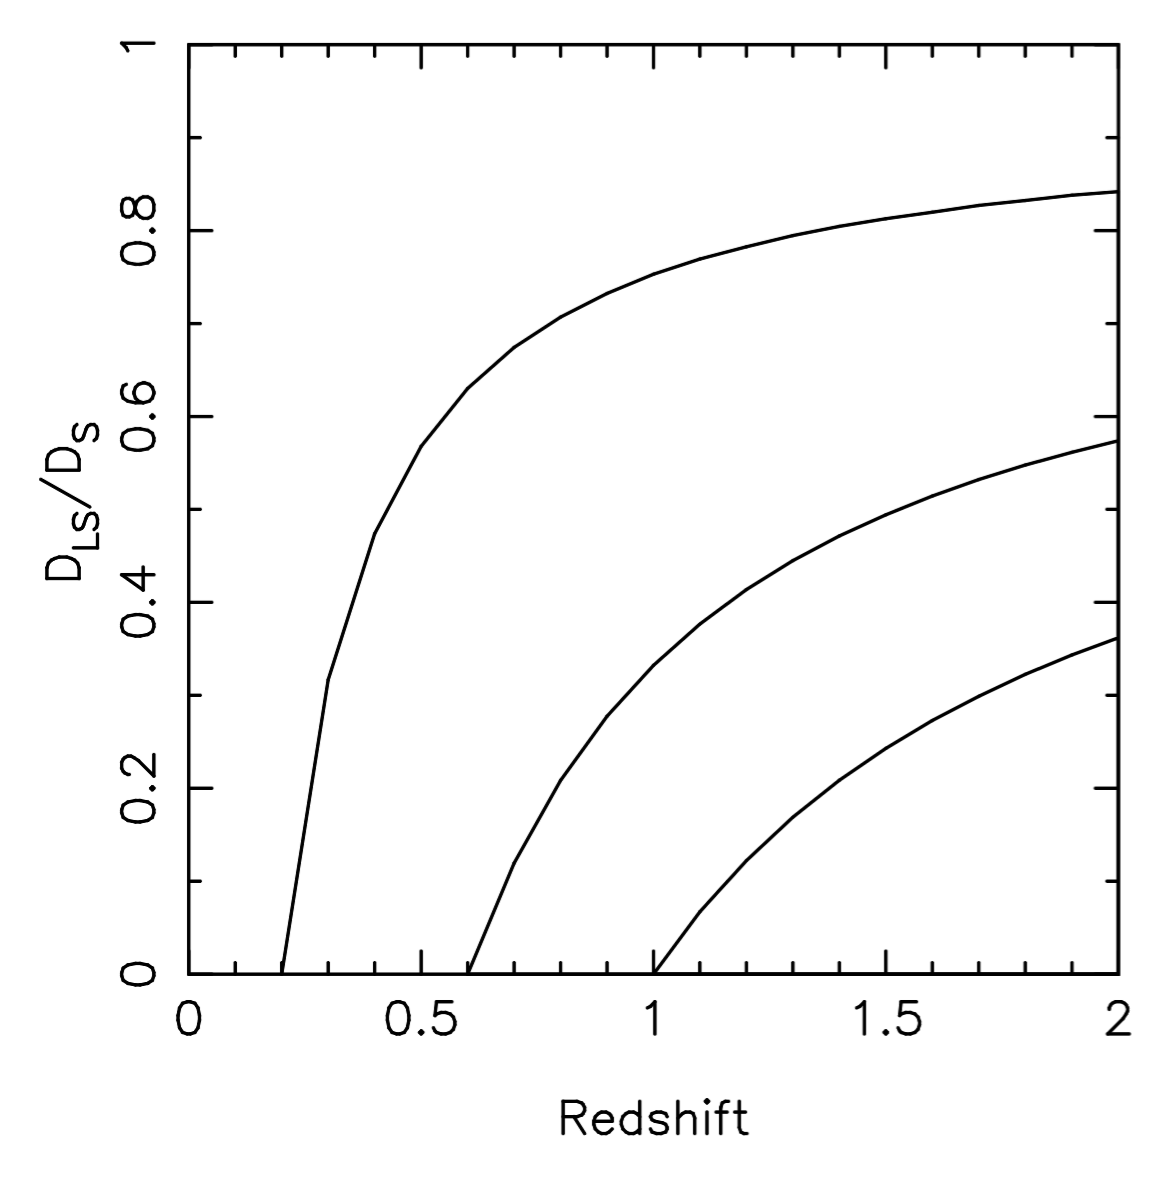
\includegraphics[width=\hsize]{dlsds.png}
\end{minipage}
\hspace{5mm}
\begin{minipage}{105mm}
  Figure~1: Dls/Ds ratio as a function of background galaxy redshift
  for cluster lenses at $z=0.2,0.6,1.0$. At any given background
  galaxy redshift the curve for the higher redshift clusters is
  steeper than the curve for lower redshift clusters.  Therefore the
  potential systematic bias due to mis-estimation of photometric
  redshifts is larger for higher redshift clusters.
\end{minipage}
%\end{figure*}

Building on the recent demonstration by Okabe \& Smith (2016) that
galaxies redder than the red sequence of cluster members in the
$(V-i)/i$ colour-magnitude plane offers a safe and calibratable method
to select galaxies behind massive galaxy clusters at $z\simeq0.2$, it
is important to explore how these methods can be extended to higher
redshifts.  Assuming for now that the rest-frame equivalents of $V$
and $i$-bands are the optimal filters for a red galaxy selection,
would motivate consideration of the $(i-J)$ colours for selection of
galaxies behind clusters at $z\simeq1$.  It is therefore clear that
photometry from \emph{Euclid} has an important role to play in
LSST-based cluster weak-lensing studies.  This point is further
amplified by the fact that merged LSST and \emph{Euclid} photometric
catalogues will be important for a broad range of extragalactic
science.  Given that this merged catalogue will be used to select
weakly-lensed background galaxies for which accurate shape
measurements are available, it is essential that the joint
LSST/\emph{Euclid} photometric catalogue production is based on the
same source identification as that used for the galaxy shape
measurement.  This begs the question of whether the source
identification for merged LSST/\emph{Euclid} photometric catalogues
should come from LSST or \emph{Euclid}?

Strategies that can be explored to improve/verify the accuracy of
photometric redshift estimates for galaxy cluster science include
choice of number, depth, and sky location of the deep drilling fields,
ultra-deep spectroscopic surveys of the deep drilling fields,
exploring how the \emph{Euclid} grism spectroscopy can assist with
spectroscopic calibration of photometric redshifts, development of
algorithms that include optical/X-ray/SZ information about the
over-densities along the line of sight through candidate clusters.

Galaxy clusters represent crowded lines of sight through the universe.
As such the requirements on the accuracy of deblended photometry are
more demanding than for typical lines of sight.  It is therefore
important to test the deblending capabilities of the LSST Data
Management team's software stack (DM Stack) on known clusters down to
$\sim5\times10^{13}M_\odot$ and out to $z\simeq1$.  It would be
sensible to do these tests on the most LSST-like data available today,
for example data obtained with Subaru telescope on massive low
redshift clusters, and also Hyper-Suprime-CAM (HSC) survey data.  On
this latter point, HSC has observed the XXL-N field to full survey
depth already.  This field contains clusters across the required
redshift and mass range.  The UK is well-placed to lead in this area
given the leading roles that we play in LoCuSS and XXL.  

\subsection{Machine learning and cluster detection methods {\it [Responsible: Jim Geach]}}

\subsection{Brightest cluster galaxies {\it [Responsible: Alastair Edge]}}


\subsection{What else? {\it [Responsible: Who else?]}}

\section{Common themes for discussion with the wider LSST community}

\subsection{Combining LSST and Euclid data products}

\subsection{Combining LSST data with the e-ROSITA cluster catalogues}

\subsection{Requirements on numerical simulations}

\subsection{Requirements on data quality including flat-fielding}

\subsection{Synergies with other Working Groups and Science Collaborations}

\subsubsection{Weak-lensing}

\subsubsection{Strong-lensing}

\subsubsection{Galaxies}

\subsubsection{Others?}

\section{Summary}


\end{document}
